%%%%%%%%%%%%%%%%%%%%%%%%%%%%%%%%%%%%%%%%%
% PREAMBLE & CONFIGURATION
%%%%%%%%%%%%%%%%%%%%%%%%%%%%%%%%%%%%%%%%%

%----------------------------------------------------------------------------------------
%   PACKAGES
%----------------------------------------------------------------------------------------
\usepackage[utf8]{inputenc} % Required for inputting international characters
\usepackage[T1]{fontenc} % Output font encoding for international characters
\usepackage{lmodern} % Scalable T1 font required for microtype expansion on this system
\usepackage[final]{microtype} % Better kerning, font expansion, and protrusion to mitigate small overfull boxes
\microtypesetup{protrusion=true, expansion=true}
\usepackage{amsmath} % Required for advanced math environments like equation*
\usepackage{amssymb} % Required for \mathbb and \checkmark
\usepackage[backend=biber, sorting=none, natbib=true]{biblatex}\usepackage[autostyle=true]{csquotes} % Required for language-dependent quotes
\usepackage{graphicx} % Required for images

% Shrink a math block to fit \linewidth only when it is too wide (never enlarge).
\newsavebox{\iseqlbox}
\newcommand{\iseqlfit}[1]{%
  \sbox{\iseqlbox}{#1}%
  \ifdim\wd\iseqlbox>\linewidth
    \resizebox{\linewidth}{!}{\usebox{\iseqlbox}}%
  \else
    \usebox{\iseqlbox}%
  \fi}

% --- TikZ for ISEQL interval diagrams
\usepackage{tikz}
\usetikzlibrary{arrows,shapes,arrows.meta,calc,math,positioning}

\tikzstyle{interval}            = [line width = 1pt, > = {Circle[length = 3.4pt]}, shorten > = -0pt]
\tikzstyle{interval label}      = [font = {\small}]

\newcommand*{\Interval}[5][]{%
    \draw[interval, #1] (#2, #4) -- (#3, #4);
    \node[interval label] at (-0.5,#4) {#5};
}

\newcommand*{\RSIntervals}[6]{%
    \Interval[#1]{#2}{#3}{1}{$r$}
    \Interval[#4]{#5}{#6}{0}{$s$}
}

\newcommand*{\DoodleSP}{%
    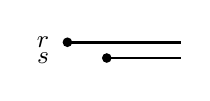
\begin{tikzpicture}[xscale=0.5, yscale=0.2, baseline={($(current bounding box.north)-(0,7.5pt)$)}]
        \RSIntervals{<-}{0}{3}{<-}{1}{3}
    \end{tikzpicture}%
}

\newcommand*{\DoodleBef}{%
    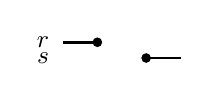
\begin{tikzpicture}[xscale=0.5, yscale=0.2, baseline={($(current bounding box.north)-(0,7.5pt)$)}]
        \RSIntervals{->}{0}{1}{<-}{2}{3}
    \end{tikzpicture}%
}

\newcommand*{\DoodleLOJ}{%
    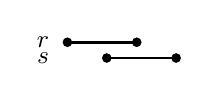
\begin{tikzpicture}[xscale=0.5, yscale=0.2, baseline={($(current bounding box.north)-(0,7.5pt)$)}]
        \RSIntervals{<->}{0}{2}{<->}{1}{3}
    \end{tikzpicture}%
}

\newcommand*{\DoodleDJ}{%
    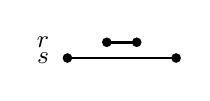
\begin{tikzpicture}[xscale=0.5, yscale=0.2, baseline={($(current bounding box.north)-(0,7.5pt)$)}]
        \RSIntervals{<->}{1}{2}{<->}{0}{3}
    \end{tikzpicture}%
}

\newcommand*{\DoodleEF}{%
    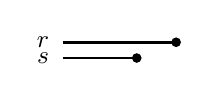
\begin{tikzpicture}[xscale=0.5, yscale=0.2, baseline={($(current bounding box.north)-(0,7.5pt)$)}]
        \RSIntervals{->}{0}{3}{->}{0}{2}
    \end{tikzpicture}%
}

% --- ISEQL temporal operators
\newcommand*{\Bef}{\mathrm{Bef}}
\newcommand*{\SP}{\mathrm{SP}}
\newcommand*{\LOJ}{\mathrm{LOJ}}
\newcommand*{\DJoin}{\mathrm{DJ}}
\newcommand*{\EF}{\mathrm{EF}}
\usepackage{siunitx} % Required for SI units
\usepackage{xurl} % Allow better URL line breaks (especially in bibliography)
\emergencystretch=2em % Relax line-breaking slightly to avoid overfull \hbox warnings
\usepackage{booktabs} % For professional-looking tables
\usepackage{pifont} % Required for \ding symbols
\newcommand{\xmark}{\text{\ding{55}}} % Cross mark symbol
\usepackage{tabularx} % For tables with automatic line wrapping
\usepackage{longtable} % For tables that span multiple pages
\usepackage{caption}  % For table captions
\usepackage{listings}
\lstset{
  basicstyle=\small\ttfamily,
  breaklines=true,
  breakatwhitespace=true,
  columns=fullflexible,
  frame=single,
  xleftmargin=2em,
  framexleftmargin=1em
}

%----------------------------------------------------------------------------------------
%   BIBLIOGRAPHY
%----------------------------------------------------------------------------------------
\addbibresource{references.bib} % The filename of the bibliography
% Improve URL line breaking in bibliography entries
\Urlmuskip=0mu plus 1mu\relax
\setcounter{biburlnumpenalty}{100}
\setcounter{biburlucpenalty}{100}
\setcounter{biburllcpenalty}{100}

%----------------------------------------------------------------------------------------
%   MARGIN SETTINGS
%----------------------------------------------------------------------------------------
\geometry{
  paper=a4paper, % Change to letterpaper for US letter
  inner=2.5cm, % Inner margin
  outer=3.8cm, % Outer margin
  bindingoffset=.5cm, % Binding offset
  top=1.5cm, % Top margin
  bottom=1.5cm, % Bottom margin
}
%----------------------------------------------------------------------------------------
%   THESIS INFORMATION
%----------------------------------------------------------------------------------------
% Update these values before you start writing.
\newcommand{\thesistypename}{Master Thesis}
\newcommand{\programmename}{Joint Degree of Master of Science in Mathematical Modelling in Engineering: Theory, Numerics, Applications}
\newcommand{\academicyear}{2026--2027}
\newcommand{\titlepagelogo}{Figures/Logos/univaq.png}
\newcommand{\titlepagepartnerlogo}{Figures/Logos/uhh.jpg}
\newcommand{\programmelogo}{Figures/Logos/mathmods.jpg}
\newcommand{\titlepagelogosize}{2.7cm}
\newcommand{\titlepagelogowidth}{4.8cm}
\newcommand{\titlepagelogoleftlabel}{UNIVERSIT\`A DEGLI STUDI DELL'AQUILA}
\newcommand{\titlepagelogorightlabel}{UNIVERSIT\"AT HAMBURG}
\newcommand{\titlepagelogolefturl}{https://www.univaq.it/en/}
\newcommand{\titlepagelogorighturl}{https://www.uni-hamburg.de/}
\newcommand{\programmeurl}{https://www.mathmods.eu/}
\newcommand{\authorurl}{https://github.com/ghiffaryr}
\newcommand{\supervisorurl}{https://www.disim.univaq.it/FabioPersia}
\newcommand{\departmenturl}{https://www.disim.univaq.it/}

\newcommand{\printtitlepagelogos}{%
  \begingroup
  \setlength{\tabcolsep}{12pt}%
  \begin{tabular}{@{}cc@{}}
    \parbox[c]{\titlepagelogowidth}{\centering
      \parbox[c][\titlepagelogosize][c]{\titlepagelogosize}{\centering\includegraphics[width=\titlepagelogosize,height=\titlepagelogosize,keepaspectratio]{\titlepagelogo}}\\[0.3cm]
      \href{\titlepagelogolefturl}{\titlepagelogoleftlabel}
    } &
    \parbox[c]{\titlepagelogowidth}{\centering
      \parbox[c][\titlepagelogosize][c]{\titlepagelogosize}{\centering\includegraphics[width=\titlepagelogosize,height=\titlepagelogosize,keepaspectratio]{\titlepagepartnerlogo}}\\[0.3cm]
      \href{\titlepagelogorighturl}{\titlepagelogorightlabel}
    }
  \end{tabular}%
  \endgroup
}

\newcommand{\printprogrammelogo}{%
  \includegraphics[width=0.4\linewidth]{\programmelogo}%
}

\thesistitle{WATCHOUT ISEQL: Large Audio-Language Models and Object Re-Identification for Forensic Multimodal Surveillance Event Detection}
\supervisor{Prof. Fabio \textsc{Persia}}
\cosupervisor{}
\degree{Master of Science}
\author{Ghiffary \textsc{Rifqialdi}}
\subject{Computer Science}
\keywords{multimodal surveillance, forensic event detection, ISEQL, large audio-language models, object re-identification, vision-language models, three-condition ablation}

\university{UNIVERSIT\`A DEGLI STUDI DELL'AQUILA\\UNIVERSIT\"AT HAMBURG}
\department{\href{\departmenturl}{Department of Information Engineering, Information Sciences and Mathematics}}
\faculty{\href{http://faculty.university.com}{Faculty Name}}

%----------------------------------------------------------------------------------------
%   PDF METADATA
%----------------------------------------------------------------------------------------
\AtBeginDocument{
  \hypersetup{pdftitle=\ttitle} % Set the PDF's title to your title
  \hypersetup{pdfauthor=\authorname} % Set the PDF's author to your name
  \hypersetup{pdfkeywords=\keywordnames} % Set the PDF's keywords to your keywords
}

%----------------------------------------------------------------------------------------
%   CUSTOM PROGRAMME PAGE ENVIRONMENT
%----------------------------------------------------------------------------------------
\newenvironment{programmepage}{
  \thispagestyle{empty} % No page number
  \begin{center}
    % Use \vfill to create flexible vertical space
    \vspace*{0.01\textheight} % A smaller fixed space from the top
    \vfill % Fill the space above the text

    {\large\textbf{This thesis was conducted within \href{\programmeurl}{\programmename}.}}\par

    \vspace{4cm} % A fixed space between the text and the logo

    \printprogrammelogo

    \vfill % Fill the remaining space at the bottom of the page
  \end{center}
  \clearpage % Automatically starts a new page after this one
}{}